\begin{figure}
  \centering
  % http://pgfplots.sourceforge.net/gallery.html
  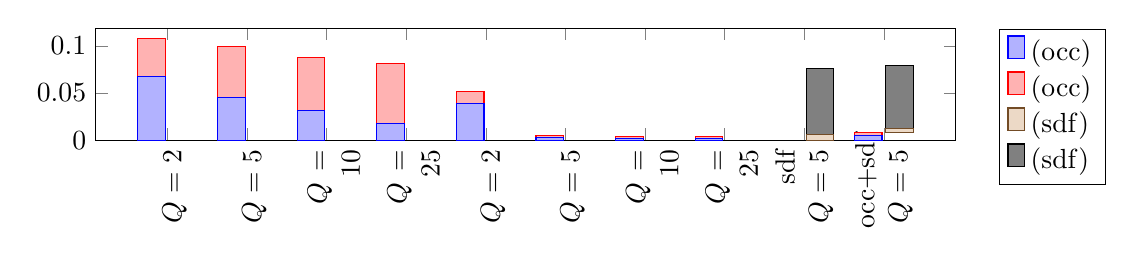
\begin{tikzpicture}
    \begin{axis}[
        ybar stacked,
        % https://tex.stackexchange.com/questions/119887/remove-the-scientific-notation-which-is-unreasonable
        yticklabel style={
          /pgf/number format/fixed,
          /pgf/number format/precision=5
        },
        scaled y ticks=false,
        legend style={
          at={(1.05,1)},
          anchor=north west,
        },
        % https://tex.stackexchange.com/questions/48620/pgfplots-alignment-and-size-of-math-in-legend
        legend cell align=left,
        % https://tex.stackexchange.com/questions/135595/how-to-correct-problem-with-ybar-plot-bad-axis-and-too-many-labels-in-x-axis
        xtick={
          1, 2, 3, 4,
          5, 6, 7, 8,
          9, 10
        },
        xticklabels={
          \PPCA\\$Q = 2$, \PPCA\\$Q = 5$, \PPCA\\$Q = 10$, \PPCA\\$Q = 25$,
          \VAE\\$Q = 2$, \VAE\\$Q = 5$, \VAE\\$Q = 10$, \VAE\\$Q = 25$,
          \VAE sdf\\$Q = 5$, \VAE occ+sdf\\$Q = 5$
        },
        x tick label style={text width=1cm,align=right},
        ymin=0,
        height=3cm,
        width=12.5cm,
        % https://tex.stackexchange.com/questions/271027/pgfplots-how-to-rotate-extra-x-tick-labels
        x tick label style={
          rotate=90,
          anchor=east,
        },
      ]
      
      % AbsThr
      \addplot +[bar shift=-.2cm] coordinates {
        (1, 0.06709765625)
        (2, 0.0449326171875)
        (3, 0.0312314453125)
        (4, 0.0177939453125)
        (5, 0.03853159)
        (6, 0.00318352)
        (7, 0.00182621)
        (8, 0.00181555)
        (9, 0)
        (10, 0.00499229)
      };
      \addlegendentry{\AbsThr (occ)}
      % Abs
      \addplot +[bar shift=-.2cm] coordinates {
        (1, 0.0404) % 0.107466870529)
        (2, 0.0542) % 0.0973753175757)
        (3, 0.05637) % 0.0876120861329)
        (4, 0.0634) % 0.0711613035139)
        (5, 0.01271) % 0.05121126)
        (6, 0.001974) % 0.00515391)
        (7, 0.001784) % 0.00361275)
        (8, 0.00185) % 0.00366516)
        (9, 0)
        (10, 0.002778) % 0.00777563)
      };
      \addlegendentry{\Abs (occ)}
      
      \resettenstackedplots
      
      %
      \addplot +[bar shift=.2cm]coordinates {
        (1, 0)
        (2, 0)
        (3, 0)
        (4, 0)
        (5, 0)
        (6, 0)
        (7, 0)
        (8, 0)
        (9, 0.00623527)
        (10, 0.00514245)
      };
      \addlegendentry{\AbsThr (sdf)}
      %
      \addplot +[bar shift=.2cm] coordinates {
        (1, 0)
        (2, 0)
        (3, 0)
        (4, 0)
        (5, 0)
        (6, 0)
        (7, 0)
        (8, 0)
        (9, 0.070219) % 0.07644901)
        (10, 0.06591859) % 0.07105859)
      };
      \addlegendentry{\Abs (sdf)}
    \end{axis}
  \end{tikzpicture}
  % TODO short caption
  \caption{Absolute error \Abs and its thresholded pendant
  \AbsThr, \ie the absolute error after thresholding the predicted shapes,
  for \PPCA and \VAE with different size $Q \in \{2,5,10,25\}$ of the
  latent space. For \VAE we additionally compare the different representations,
  \ie occupancy (occ) and signed distance functions (sdf). For \PPCA we only
  report results on occupancy. Note that
  for \VAEs and occupancy, \Abs and \AbsThr are usually very close together.
  In each case, the bars on the left represent result son occupancy (if applicable);
  while the bars on the right correspond to results on signed distance functions
  (if applicable).}
  \label{fig:experiments-2d-ppca}
\end{figure}
